\documentclass[../piano-di-qualifica.tex]{subfiles}


\begin{document}
  \subsection{Analisi statica dei documenti}%
  \label{sub:analisi_statica_doc}
	Per l'analisi statica dei documenti GruppOne ha utilizzato il package \glossario{chktex} che ha consentito di trovare errori nella sintassi latex.
  Il test, eseguito ad ogni modifica repository, ha dato esito positivo per ogni documento segnalando complessivamente 0 errori.

  \begin{figure}[H]
    \centering
    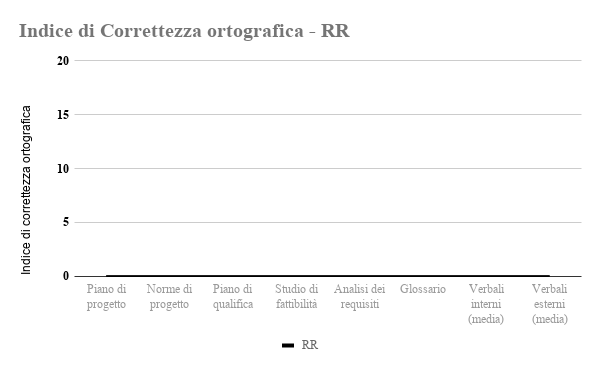
\includegraphics[width=160mm]{correttezzaortografica-RR.png}%
  \end{figure}


  \begin{figure}[H]
    \centering
    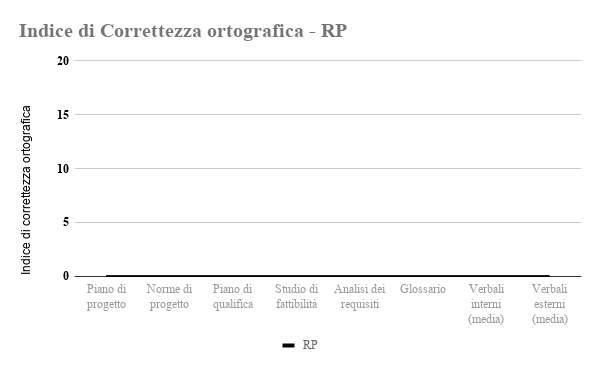
\includegraphics[width=160mm]{correttezzaortografica-RP.png}%
  \end{figure}



	% sub:analisi_statica_doc (end)
  \subsection{Esito verifica leggibilità}%
  \label{sub:verifica_leggibilita}
	Allo scopo di assicurarci una leggibilità accettabile dei documenti abbiamo monitorato l'indice \glossario{Gulpease} di ogni documento. Qui sotto riportiamo i risultati della versione consegnata in RR e successive relativamente agli obiettivi di qualità che erano stati definiti.
  \rowcolors{2}{lightgray}{white!80!lightgray!100}
  \begin{longtable}[H]{>{\centering\bfseries}m{6cm} >{\centering\arraybackslash}m{2cm} >{\centering\arraybackslash}m{2cm}>{\centering\arraybackslash}m{2cm} >{\centering\arraybackslash}m{4cm}}
    \rowcolor{darkgray!90!}
    \color{white}{\textbf{Documento}} & \color{white}{\textbf{RR}} & \color{white}{\textbf{RP}} &\color{white}{\textbf{Esito dell'ultima verifica}} \\
    Piano di Progetto & 96 & 95&Sufficiente\\
    Norme di Progetto & 68 & 74&Sufficiente\\
    Piano di Qualifica & 81 & 83&Sufficiente\\
    Studio di Fattibilità & 65 & -&Sufficiente\\
    Analisi dei requisiti & 100 & 100&Sufficiente\\
    Glossario & 74 & 83& Sufficiente\\
    Verbale esterno (media) & 77 & 74&Sufficiente \\
    Verbale interno (media) & 80 & 77&Sufficiente\\
\end{longtable}
\begin{figure}[H]
  \centering
  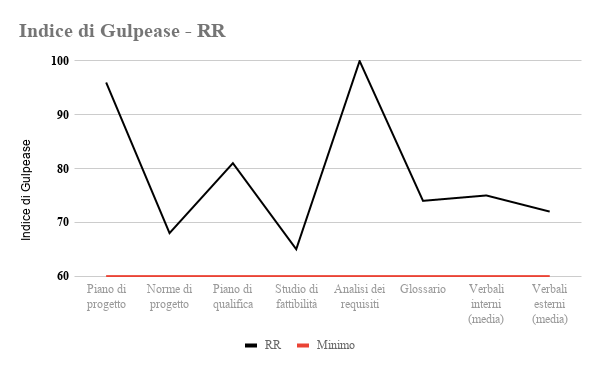
\includegraphics[width=160mm]{gulpease-RR.png}%
\end{figure}

\begin{figure}[H]
  \centering
  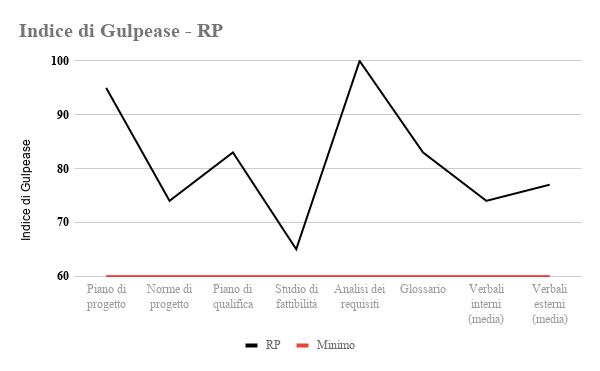
\includegraphics[width=160mm]{gulpease-RP.png}%
\end{figure}


\begin{figure}[H]
  \centering
  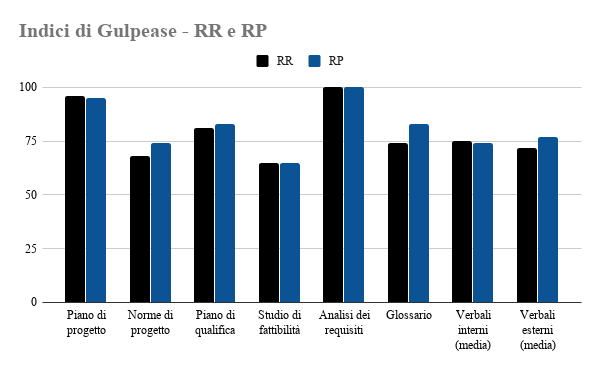
\includegraphics[width=160mm]{gulpease-conf.png}%
\end{figure}

	% sub:verifica_leggibilita (end)
\end{document}

\subsection{Discostamenti orari ed economici}%
\label{sub:discostamenti_orari_ed_economici}
Per assicurarci di rispettare il preventivo, abbiamo monitorato i discostamenti, in percentuale, fra ila lavoro eseguito e quello pianificato, dai punti di vista economico ed orario. Nel seguito riportiamo i risultati al termine di ogni fase.

\begin{figure}[H]
  \centering
  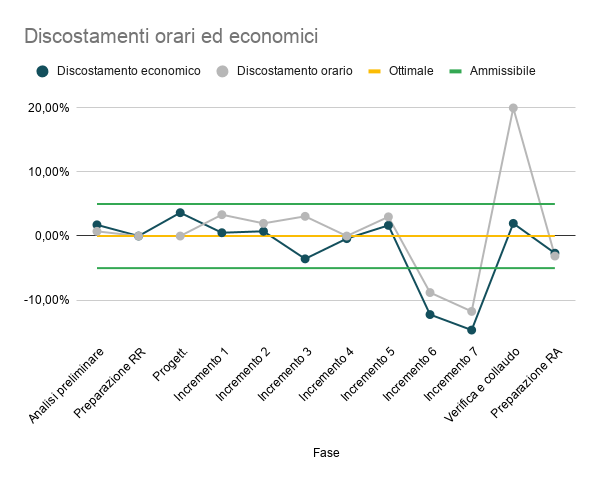
\includegraphics[width=160mm]{discostamenti-orari-economici.png}%
  \caption{Discostamenti orari ed economici, in percentuale}%
\end{figure}
% sub:discostamenti_orari_ed_economici (end)
